\documentclass[border=25pt]{standalone}
\usepackage{tikz}
\usetikzlibrary{positioning, fit, arrows.meta, calc, backgrounds, decorations.pathreplacing}
\usepackage{amsmath, amssymb}

\begin{document}
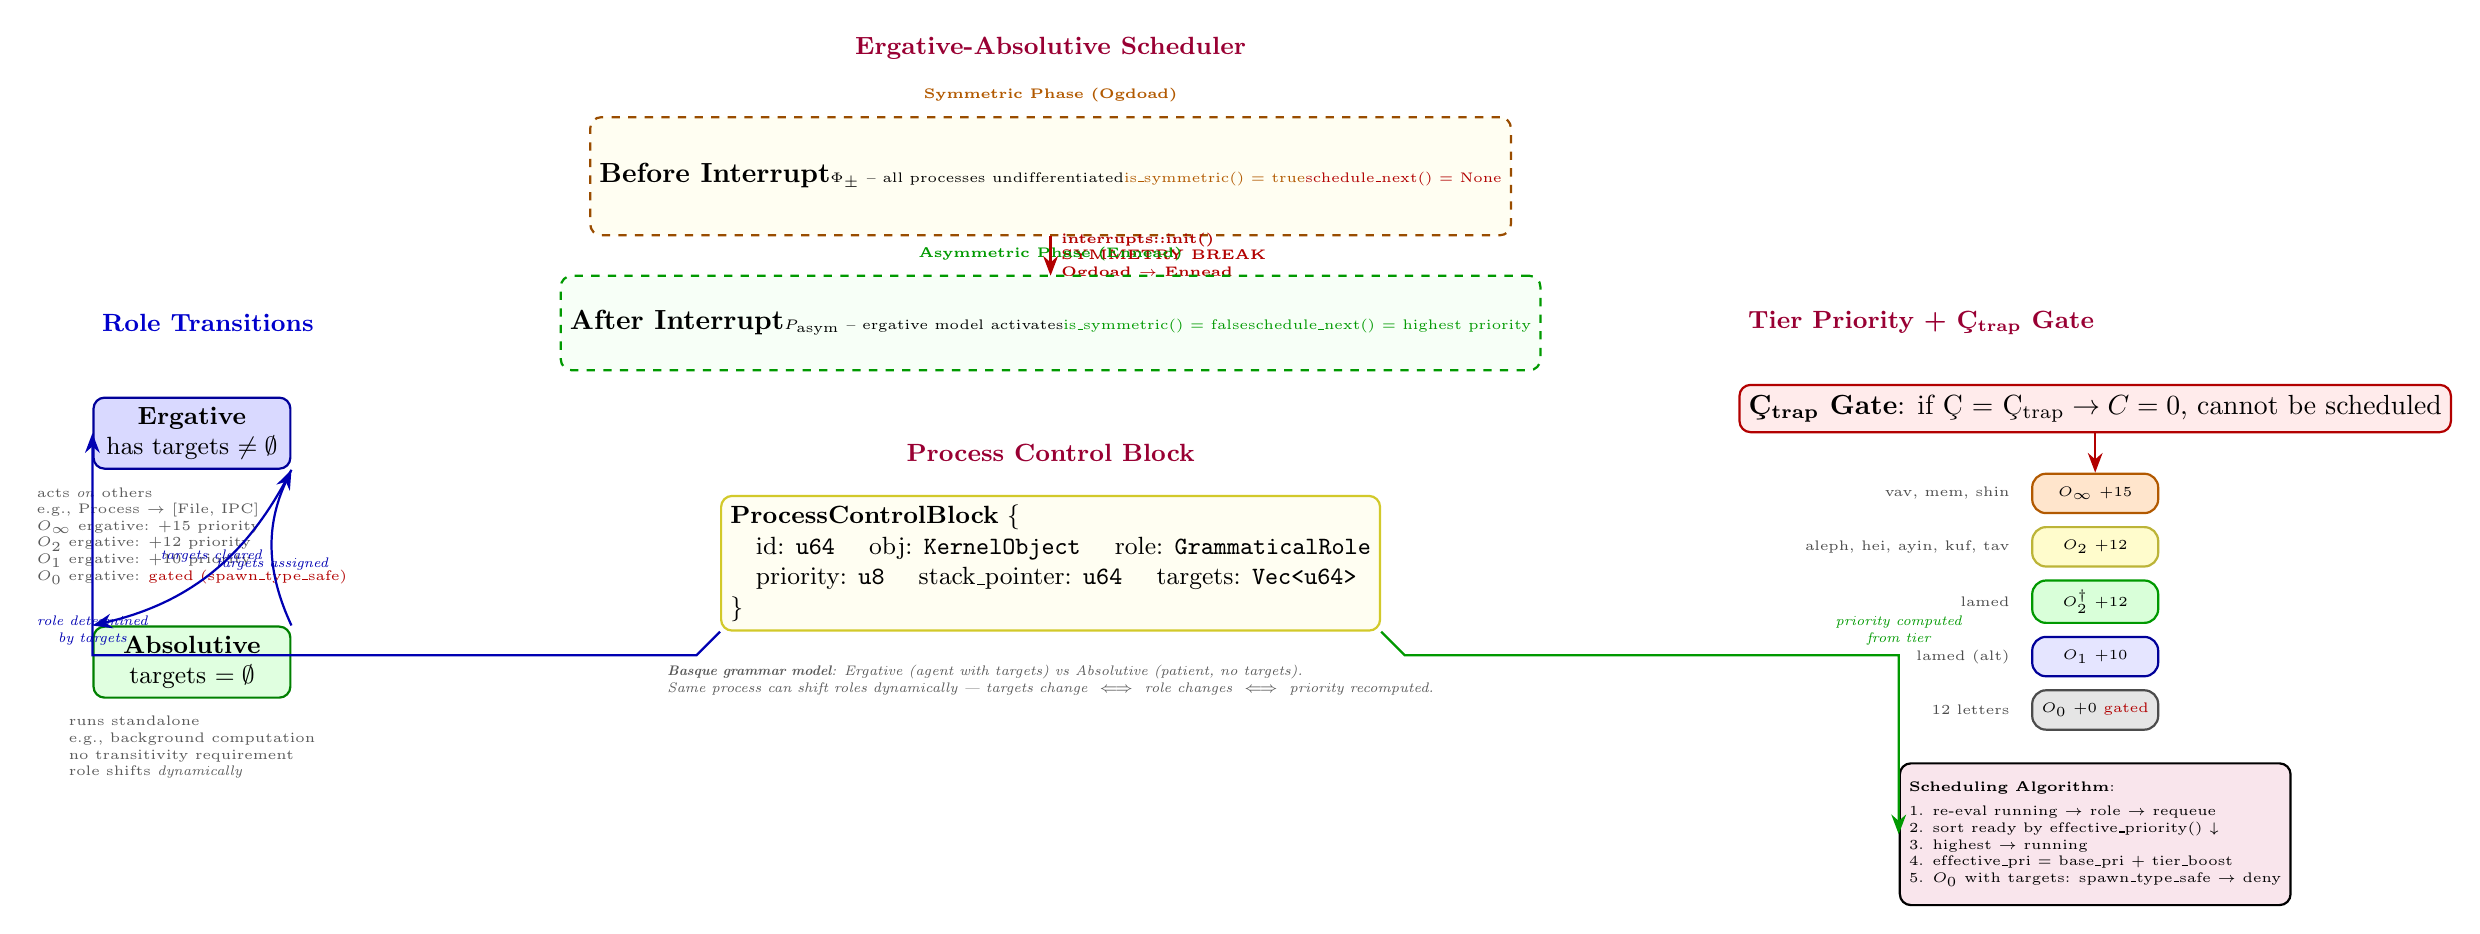
\begin{tikzpicture}[
  node distance=0.5cm and 1.2cm,
  proc/.style={rectangle, draw, thick, rounded corners, minimum width=2.5cm, minimum height=0.6cm, align=center, font=\small},
  erg/.style={proc, fill=blue!15, draw=blue!60!black},
  abs/.style={proc, fill=green!12, draw=green!50!black},
  trap/.style={proc, fill=red!15, draw=red!60!black},
  tier/.style={rectangle, draw, thick, rounded corners=5pt, minimum width=1.6cm, minimum height=0.5cm, align=center, font=\tiny},
  arrow/.style={-{Stealth[length=2.5mm]}, thick, yellow!60!black},
  arrow_b/.style={-{Stealth[length=2.5mm]}, thick, blue!70!black},
  arrow_g/.style={-{Stealth[length=2.5mm]}, thick, green!60!black},
  arrow_r/.style={-{Stealth[length=2.5mm]}, thick, red!70!black},
  arrow_o/.style={-{Stealth[length=2.5mm]}, thick, orange!70!black},
  labeln/.style={font=\tiny\itshape, align=center},
  symbox/.style={draw=orange!60!black, thick, dashed, rounded corners, fill=yellow!5}
]

% ============================================================
% TOP: Symmetry State
% ============================================================
\node[font=\bfseries\small, text=purple!80!black] (title) {Ergative-Absolutive Scheduler};

% Before symmetry break
\node[symbox, minimum width=4.5cm, minimum height=1.5cm, below=0.6cm of title] (sym) {
  \textbf{Before Interrupt} \\
  \tiny $\Phi_{\pm}$ -- all processes undifferentiated \\
  \tiny \textcolor{orange!70!black}{is\_symmetric() = true} \\
  \tiny \textcolor{red!70!black}{schedule\_next() = None}
};
\node[font=\tiny\bfseries, text=orange!70!black, above=0.05cm of sym.north, anchor=south] (symlabel) {Symmetric Phase (Ogdoad)};

% Symmetry breaking arrow
\draw[arrow_r, line width=1.2pt] (sym.south) -- ++(0,-0.5)
  node[midway, right, font=\tiny\bfseries, text=red!70!black, align=left] {interrupts::init()\\SYMMETRY BREAK\\Ogdoad $\to$ Ennead};

% After symmetry break
\coordinate (asym_pos) at ($(sym.south) + (0,-1.1)$);
\node[rectangle, draw=green!60!black, thick, dashed, rounded corners, fill=green!3,
      minimum width=4.5cm, minimum height=1.2cm, at=(asym_pos)] (asym) {
  \textbf{After Interrupt} \\
  \tiny $P_{\text{asym}}$ -- ergative model activates \\
  \tiny \textcolor{green!60!black}{is\_symmetric() = false} \\
  \tiny \textcolor{green!60!black}{schedule\_next() = highest priority}
};
\node[font=\tiny\bfseries, text=green!60!black, above=0.05cm of asym.north, anchor=south] (asymlabel) {Asymmetric Phase (Ennead)};

% ============================================================
% LEFT: Role Transitions
% ============================================================
\node[font=\bfseries\small, text=blue!80!black, left=3cm of asym.west, anchor=east] (rtitle) {Role Transitions};

% Ergative process
\node[erg, below=0.7cm of rtitle.south west, anchor=north west] (erg1) {\textbf{Ergative}\\has targets $\neq \emptyset$};
\node[font=\tiny, below=0.1cm of erg1, align=left, text=gray!70!black] (erg_desc) {
  acts \emph{on} others\\
  e.g., Process $\to$ [File, IPC]\\
  $O_{\infty}$ ergative: +15 priority\\
  $O_2$ ergative: +12 priority\\
  $O_1$ ergative: +10 priority\\
  $O_0$ ergative: \textcolor{red!70!black}{gated (spawn\_type\_safe)}
};

% Absolutive process
\node[abs, below=0.4cm of erg_desc] (abs1) {\textbf{Absolutive}\\targets $= \emptyset$};
\node[font=\tiny, below=0.1cm of abs1, align=left, text=gray!70!black] (abs_desc) {
  runs standalone\\
  e.g., background computation\\
  no transitivity requirement\\
  role shifts \emph{dynamically}
};

% Transition arrows
\draw[arrow_b, bend left=25] (erg1.south east) to node[above, labeln] {targets cleared} (abs1.north west);
\draw[arrow_b, bend left=25] (abs1.north east) to node[below, labeln] {targets assigned} (erg1.south east);

% ============================================================
% RIGHT: Tier Priority + Ç_trap Gate
% ============================================================
\node[font=\bfseries\small, text=purple!80!black, right=2.5cm of asym.east, anchor=west] (ttitle) {Tier Priority + Ç$_{\text{trap}}$ Gate};

% Ç_trap gate
\node[rectangle, draw=red!70!black, thick, rounded corners, fill=red!8, minimum width=3.5cm, minimum height=0.6cm,
      below=0.5cm of ttitle.south west, anchor=north west] (ktrap) {
  \textbf{Ç$_{\text{trap}}$ Gate}: if Ç = Ç$_{\text{trap}} \to C = 0$, cannot be scheduled
};

% Tier priority ladder
\node[tier, fill=orange!20, draw=orange!70!black, below=0.5cm of ktrap] (tinf) {$O_{\infty}$ +15};
\node[tier, fill=yellow!20, draw=yellow!70!black, below=0.15cm of tinf] (t2) {$O_2$ +12};
\node[tier, fill=green!15, draw=green!60!black, below=0.15cm of t2] (t2d) {$O_{2}^{\dagger}$ +12};
\node[tier, fill=blue!10, draw=blue!60!black, below=0.15cm of t2d] (t1) {$O_1$ +10};
\node[tier, fill=gray!20, draw=gray!60!black, below=0.15cm of t1] (t0) {$O_0$ +0 \textcolor{red!70!black}{gated}};

% Letters per tier
\node[font=\tiny, left=0.15cm of tinf.west, anchor=east, text=gray!60!black] {vav, mem, shin};
\node[font=\tiny, left=0.15cm of t2.west, anchor=east, text=gray!60!black] {aleph, hei, ayin, kuf, tav};
\node[font=\tiny, left=0.15cm of t2d.west, anchor=east, text=gray!60!black] {lamed};
\node[font=\tiny, left=0.15cm of t1.west, anchor=east, text=gray!60!black] {lamed (alt)};
\node[font=\tiny, left=0.15cm of t0.west, anchor=east, text=gray!60!black] {12 letters};

% Scheduling algorithm
\node[rectangle, draw, thick, rounded corners, fill=purple!10, minimum width=3.5cm, minimum height=1.8cm,
      below=0.4cm of t0, align=left, font=\tiny] (algo) {
  \textbf{Scheduling Algorithm}:\\[0.1cm]
  1. re-eval running $\to$ role $\to$ requeue\\
  2. sort ready by effective\_priority() $\downarrow$\\
  3. highest $\to$ running\\
  4. effective\_pri = base\_pri + tier\_boost\\
  5. $O_0$ with targets: spawn\_type\_safe $\to$ deny
};

% ============================================================
% BOTTOM: Process Control Block
% ============================================================
\node[font=\bfseries\small, text=purple!80!black, below=0.8cm of asym.south, anchor=north] (pcbtitle) {Process Control Block};

\node[rectangle, draw=yellow!80!black, thick, rounded corners, fill=yellow!5, minimum width=8cm, minimum height=1.5cm,
      below=0.3cm of pcbtitle, align=left, font=\small] (pcb) {
  \textbf{ProcessControlBlock} \{ \\
  \quad id: \texttt{u64} \quad obj: \texttt{KernelObject} \quad role: \texttt{GrammaticalRole} \\
  \quad priority: \texttt{u8} \quad stack\_pointer: \texttt{u64} \quad targets: \texttt{Vec<u64>} \\
  \}
};

% Connections
\draw[arrow_b] (pcb.south west) -- ++(-0.3,-0.3) -| (erg1.west)
  node[midway, above, labeln] {role determined\\by targets};
\draw[arrow_g] (pcb.south east) -- ++(0.3,-0.3) -| (algo.west)
  node[midway, above, labeln] {priority computed\\from tier};
\draw[arrow_r] (ktrap.south) -- (tinf.north);

% Bottom note
\node[below=0.3cm of pcb, align=left, font=\tiny\itshape, text=gray!70!black] (note) {
  \textbf{Basque grammar model}: Ergative (agent with targets) vs Absolutive (patient, no targets). \\
  Same process can shift roles dynamically --- targets change $\iff$ role changes $\iff$ priority recomputed.
};

\end{tikzpicture}
\end{document}